\documentclass[letter, 10pt]{article}
\usepackage[latin1]{inputenc}
\usepackage[spanish]{babel}
\usepackage{amsfonts}
\usepackage{amsmath}
\usepackage[pdftex]{graphicx}
%\usepackage[dvips]{graphicx}
\usepackage{url}
\usepackage[top=3cm,bottom=3cm,left=3.0cm,right=3.0cm,footskip=1.5cm,headheight=1.5cm,headsep=.5cm,textheight=3cm]{geometry}
\usepackage{moreverb}

\let\verbatiminput=\verbatimtabinput


\begin{document}
\title{Investigaci�n de Operaciones I \\
	\begin{Large}Tarea 2: Programaci�n y Control de
	Proyectos\end{Large}}
\author{Cristian Maureira \\ 2673030-9 \\ \texttt{cmaureir@inf.utfsm.cl} \and
	Gabriel Zamora \\ 2673070-8 \\ \texttt{gzamora@inf.utfsm.cl}}
\date{\today}
\maketitle

\section{Desarrollo}

\begin{enumerate}
	\item Malla del proyecto\\
		\begin{center}
		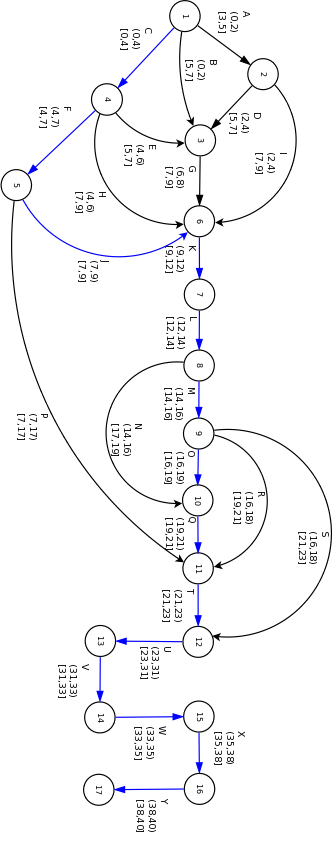
\includegraphics[height=13cm]{malla.png}
		\end{center}
	\newpage
	\item Resoluci�n gr�fica:
		\begin{itemize}
			\item Duraci�n m�nima del proyecto: 40 Semanas 
			\item Tiempo m�s temprano y m�s tarde de los sucesos\\
				\begin{tabular}{|l|l|l|}
				\hline
				Actividad & Tiempo m�s temprano & Tiempo m�s tarde\\
				\hline
				A &	(0,2)&	 [3,5] \\	
				\hline
				B &	(0,2)&   [5,7] \\	
				\hline
				C &	(0,4)&   [0,4] \\	
				\hline
				D &	(2,4)&   [5,7] \\	
				\hline
				E &	(4,6)&   [5,7] \\	
				\hline
				F &	(4,7)&   [4,7] \\	
				\hline
				G &	(6,8)&   [7,9] \\	
				\hline
				H &	(4,6)&   [7,9] \\	
				\hline
				I &	(2,4)&   [7,9] \\	
				\hline
				J &	(7,9)&   [7,9] \\	
				\hline
				K &	(9,12)&  [9,12] \\	
				\hline
				L &	(12,14)& [12,14] \\	
				\hline
				M &	(14,16)& [14,16] \\	
				\hline
				N &	(14,16)& [17,19] \\	
				\hline
				O &	(16,19)& [16,19] \\	
				\hline
				P &	(7,17)&  [11,21] \\	
				\hline
				Q &	(19,21)& [19,21] \\	
				\hline
				R &	(16,18)& [19,21] \\	
				\hline
				S &	(16,18)& [21,23] \\	
				\hline
				T &	(21,23)& [21,23] \\	
				\hline
				U &	(23,31)& [23,31] \\	
				\hline
				V &	(31,33)& [31,33] \\	
				\hline
				W &	(33,35)& [33,35] \\	
				\hline
				X &	(35,38)& [35,38] \\
				\hline
				Y &	(38,40)& [38,40] \\
				\hline
				\end{tabular}
			\item Ruta(s) cr�tica(s):\\
				C-F-J-K-L-M-O-Q-T-U-V-W-X-Y				
		\end{itemize}
	\newpage
	\item Resoluci�n con Programaci�n Lineal
		\begin{itemize}
			\item Modelo LP
				\begin{itemize}
					\item Variables:\\
						$X_i$: Tiempo acumulado hasta el nodo i, i = {1, $\ldots$, 17}\\
						$t_{i\_j}$: Tiempo que demoran en realizarse la actividad entre el nodo i hasta el nodo j\\
					\item Funci�n Objetivo:\\
						M�nimo $Z = X_{17} - X_1$
					\item Restricciones:\\
						\begin{itemize}
							\item Tiempos:\\
								$X_{2 } \geq  X_{1 } + t_{1\_2}   =  X_{2 } +  2 $\\
								$X_{3 } \geq  X_{1 } + t_{1\_3}   =  X_{3 } +  2 $\\
								$X_{4 } \geq  X_{1 } + t_{1\_4}   =  X_{4 } +  4 $\\
								$X_{3 } \geq  X_{2 } + t_{2\_3}   =  X_{3 } +  2 $\\
								$X_{3 } \geq  X_{4 } + t_{4\_3}   =  X_{3 } +  2 $\\
								$X_{5 } \geq  X_{4 } + t_{4\_5}   =  X_{5 } +  3 $\\
								$X_{6 } \geq  X_{2 } + t_{2\_6}   =  X_{6 } +  2 $\\
								$X_{6 } \geq  X_{3 } + t_{3\_6}   =  X_{6 } +  2 $\\
								$X_{6 } \geq  X_{4 } + t_{4\_6}   =  X_{6 } +  2 $\\
								$X_{6 } \geq  X_{5 } + t_{5\_6}   =  X_{6 } +  2 $\\
								$X_{7 } \geq  X_{6 } + t_{6\_7}   =  X_{7 } +  3 $\\
								$X_{8 } \geq  X_{7 } + t_{7\_8}   =  X_{8 } +  2 $\\
								$X_{9 } \geq  X_{8 } + t_{8\_9}   =  X_{9 } +  2 $\\
								$X_{10} \geq  X_{8 } + t_{8\_10}  =  X_{10} +  2 $\\
								$X_{10} \geq  X_{9 } + t_{9\_10}  =  X_{10} +  3 $\\
								$X_{11} \geq  X_{5 } + t_{5\_11}  =  X_{11} +  10$\\
								$X_{11} \geq  X_{9 } + t_{9\_11}  =  X_{11} +  2 $\\
								$X_{11} \geq  X_{10} + t_{10\_11} =  X_{11} +  2 $\\
								$X_{12} \geq  X_{9 } + t_{9\_12}  =  X_{12} +  2 $\\
								$X_{12} \geq  X_{11} + t_{11\_12} =  X_{12} +  2 $\\
								$X_{13} \geq  X_{12} + t_{12\_13} =  X_{13} +  8 $\\
								$X_{14} \geq  X_{13} + t_{13\_14} =  X_{14} +  2 $\\
								$X_{15} \geq  X_{14} + t_{14\_15} =  X_{15} +  2 $\\
								$X_{16} \geq  X_{15} + t_{15\_16} =  X_{16} +  3 $\\
								$X_{17} \geq  X_{16} + t_{16\_17} =  X_{17} +  2 $\\
							\item Naturaleza:\\
								$0 \leq X_i, i = \{1, \ldots, 17\}$
						\end{itemize}
				\end{itemize}
			\item Resoluci�n con LINDO. Comentarios
				\begin{itemize}
					\item C�digo
						\verbatiminput{modelo.ltx}
					\item Resultados\\
						\begin{tabular}{|l|l|}
							\hline
							X1 & 0 \\
							\hline
							X2 & 2 \\
							\hline
							X3 & 6 \\
							\hline
							X4 & 4 \\
							\hline
							X5 & 7 \\
							\hline
							X6 & 9 \\
							\hline
							X7 & 12 \\
							\hline
							X8 & 14 \\
							\hline
							X9 & 16 \\
							\hline
							X10 & 19 \\
							\hline
							X11 & 21 \\
							\hline
							X12 & 23 \\
							\hline
							X13 & 31 \\
							\hline
							X14 & 33 \\
							\hline
							X15 & 35 \\
							\hline
							X16 & 38 \\
							\hline
							X17 & 40 \\
							\hline
						\end{tabular}
				\end{itemize}
		\end{itemize}
	\newpage
	\item Probabilidad de que el proyecto termine antes de 29 semanas y despu�s de 48 semanas\\
		Primero que todo debemos tener claro el valor de la \emph{varianza} en cada actividad.
		Por lo tanto mediante la siguiente f�rmula, procederemos a calcular cada una.
		$$V[T_{ij}]\ =\ \frac{(b\ -\ a)^{2}}{36}$$
		Y la esperanza tambi�n es posible calcularla de acuerdo a la siguiente f�rmula:
		$$E[T_{ij}]\ =\ \frac{(a\ +\ 4m\ +\ b)}{6}$$
		Con $T_{ij}$ como la variable aleatoria asociada a la duraci�n de la actividad $(i,j)$.
		\begin{center}
			\begin{tabular}{|c|c|c|c|c|c|}
				\hline
				Actividad & a & m & b & Varianza & Esperanza \\\hline
				A & 1 & 2  & 3 & 0.1  &  2 \\\hline 
				B & 1 & 2  & 3 & 0.1  &  2 \\\hline 
				C & 2 & 4  & 6 & 0.4  &  4 \\\hline  
				D & 1 & 2  & 3 & 0.1  &  2 \\\hline 
				E & 1 & 2  & 3 & 0.1  &  2 \\\hline 
				F & 2 & 3  & 5 & 0.25 &  3 \\\hline 
				G & 1 & 2  & 3 & 0.1  &  2 \\\hline 
				H & 1 & 2  & 3 & 0.1  &  2 \\\hline 
				I & 1 & 2  & 3 & 0.1  &  2 \\\hline 
				J & 1 & 2  & 4 & 0.25 &  2 \\\hline 
				K & 2 & 3  & 5 & 0.25 &  3 \\\hline 
				L & 1 & 2  & 3 & 0.1  &  2 \\\hline 
				M & 1 & 2  & 3 & 0.1  &  2 \\\hline 
				N & 1 & 2  & 3 & 0.1  &  2 \\\hline 
				O & 2 & 3  & 4 & 0.1  &  3 \\\hline 
				P & 8 & 10 & 11& 0.25 &  9 \\\hline 
				Q & 1 & 2  & 3 & 0.1  &  2 \\\hline 
				R & 1 & 2  & 3 & 0.1  &  2 \\\hline 
				S & 1 & 2  & 3 & 0.1  &  2 \\\hline 
				T & 1 & 2  & 3 & 0.1  &  2 \\\hline 
				U & 6 & 8  & 9 & 0.25 &  7 \\\hline 
				V & 1 & 2  & 3 & 0.1  &  2 \\\hline 
				W & 1 & 2  & 4 & 0.25 &  2 \\\hline 
				X & 2 & 3  & 4 & 0.1  &  3 \\\hline 
				Y & 1 & 2  & 3 & 0.1  &  2 \\\hline 
			\end{tabular}
		\end{center}	
		Tenemos que tomar el camino critico, sumar todas las varianzas asociadas a las actividades
		del mismo camino y con eso obtenemos la varianza del proyecto:
		\begin{eqnarray}
			\sum_{(i,j)\in ruta} V[T_{ij}]  &=& V_{C}+V_{F}+V_{J}+V_{K}+V_{L}+V_{M}+V_{O}+V_{Q}+V_{T}+V_{U}+V_{V}+V_{W}+V_{X}+V_{Y} \nonumber\\
							&=& 0.4  +0.25 +0.25 +0.25 +0.1  +0.1  +0.1  +0.1  +0.1  +0.25 +0.1  +0.25 +0.1  + 0.1 \nonumber\\
							&=& 2.45\ (semanas)\nonumber\\
							&=& \sigma_{T}^{2}\ (desviacion\ estandar) \nonumber
		\end{eqnarray}
		Por lo tanto $\sigma_{T} = \sqrt{2.45} = 1.565$
		De la misma forma, obtenemos la esperanza del camino:
		\begin{eqnarray}
			\sum_{(i,j)\in ruta} E[T_{ij}]  &=& E_{C}+E_{F}+E_{J}+E_{K}+E_{L}+E_{M}+E_{O}+E_{Q}+E_{T}+E_{U}+E_{V}+E_{W}+E_{X}+E_{Y} \nonumber\\
							&=& 4    +3    +2     +3    +2    +2    +3    +2    +2    +7    +2    +2    +3    +2     \nonumber\\
							&=& 39\ (semanas)\nonumber
		\end{eqnarray}
		Para cada caso:
		\begin{itemize}
			\item Antes de 29 semanas:\\
				\begin{eqnarray}
					P(T \leq 29) &=& P(\frac{T-E{T}}{\sigma_{T}} \leq z = \frac{29 - E(T)}{\sigma_{T}} )\\
						     &=& P(\frac{T-39}{1.565} \leq  \frac{29 - 39}{1.565} )\\
						     &=& P(z \leq -6.389 )\\
						     &=& 0\% (Viendo\ una\ tabla\ normal)\\
				\end{eqnarray}
			\item Despu�s de 48 semanas:\\
				\begin{eqnarray}
					P(T \geq 48) &=& 1 - P(T \leq 48)\\
						     &=& 1 - P(\frac{T-E{T}}{\sigma_{T}} \leq z = \frac{48 - E(T)}{\sigma_{T}} )\\
						     &=& 1 - P(\frac{T-39}{1.565} \leq \frac{48-39}{1.565}\\
						     &=& 1 - P(z \leq 5.750)\\
						     &=& 0\% (Viendo\ una tabla\ normal,\ el\ valor\ es\ muy\ chico)\\
				\end{eqnarray}
		\end{itemize}
	\newpage
		\begin{itemize}
			\item Modelo LP Acelerado
				\begin{itemize}
					\item Variables:\\
						$X_i$: Tiempo acumulado hasta el nodo i, i = {1, $\ldots$, 17}\\
						$t_{i\_j}$: Tiempo que demoran en realizarse la actividad entre el nodo i hasta el nodo j\\
						$a_{i\_j}$: Tiempo m�ximo en que es posible acelerar la actividad entre el nodo i hasta el nodo j\\
					\item Funci�n Objetivo:\\
						M�nimo $Z = 100 a_{1\_2} + 50 a_{1\_3} + 300 a_{1\_4} + 100 a_{2\_3} + 500 a_{4\_3} + 50 a_{4\_5} + 150 a_{2\_6} + 70 a_{3\_6} + 60 a_{4\_6} + 350 a_{5\_6} + 20 a_{6\_7} + 80 a_{7\_8} + 40 a_{8\_9} + 230 a_{8\_10} + 10 a_{9\_10} + 30 a_{5\_11} + 500 a_{9\_11} + 100 a_{10\_11} + 20 a_{9\_12} + 140 a_{11\_12} + 200 a_{12\_13} + 45 a_{13\_14} + 100 a_{14\_15} + 150 a_{15\_16} + 200 a_{16\_17}$
					\item Restricciones:\\
						\begin{itemize}
							\item Tiempos:\\
								$X_{2 } \geq  X_{1 } + t_{1\_2}   - a_{1\_2}   = X_{1 } +  2  - a_{1\_2}   $\\
								$X_{3 } \geq  X_{1 } + t_{1\_3}   - a_{1\_3}   = X_{1 } +  2  - a_{1\_3}   $\\
								$X_{4 } \geq  X_{1 } + t_{1\_4}   - a_{1\_4}   = X_{1 } +  4  - a_{1\_4}   $\\
								$X_{3 } \geq  X_{2 } + t_{2\_3}   - a_{2\_3}   = X_{2 } +  2  - a_{2\_3}   $\\
								$X_{3 } \geq  X_{4 } + t_{4\_3}   - a_{4\_3}   = X_{4 } +  2  - a_{4\_3}   $\\
								$X_{5 } \geq  X_{4 } + t_{4\_5}   - a_{4\_5}   = X_{4 } +  3  - a_{4\_5}   $\\
								$X_{6 } \geq  X_{2 } + t_{2\_6}   - a_{2\_6}   = X_{2 } +  2  - a_{2\_6}   $\\
								$X_{6 } \geq  X_{3 } + t_{3\_6}   - a_{3\_6}   = X_{3 } +  2  - a_{3\_6}   $\\
								$X_{6 } \geq  X_{4 } + t_{4\_6}   - a_{4\_6}   = X_{4 } +  2  - a_{4\_6}   $\\
								$X_{6 } \geq  X_{5 } + t_{5\_6}   - a_{5\_6}   = X_{5 } +  2  - a_{5\_6}   $\\
								$X_{7 } \geq  X_{6 } + t_{6\_7}   - a_{6\_7}   = X_{6 } +  3  - a_{6\_7}   $\\
								$X_{8 } \geq  X_{7 } + t_{7\_8}   - a_{7\_8}   = X_{7 } +  2  - a_{7\_8}   $\\
								$X_{9 } \geq  X_{8 } + t_{8\_9}   - a_{8\_9}   = X_{8 } +  2  - a_{8\_9}   $\\
								$X_{10} \geq  X_{8 } + t_{8\_10}  - a_{8\_10}  = X_{8 } +  2  - a_{8\_10}  $\\
								$X_{10} \geq  X_{9 } + t_{9\_10}  - a_{9\_10}  = X_{9 } +  3  - a_{9\_10}  $\\
								$X_{11} \geq  X_{5 } + t_{5\_11}  - a_{5\_11}  = X_{5 } +  10 - a_{5\_11}  $\\
								$X_{11} \geq  X_{9 } + t_{9\_11}  - a_{9\_11}  = X_{9 } +  2  - a_{9\_11}  $\\
								$X_{11} \geq  X_{10} + t_{10\_11} - a_{10\_11} = X_{10} +  2  - a_{10\_11} $\\
								$X_{12} \geq  X_{9 } + t_{9\_12}  - a_{9\_12}  = X_{9 } +  2  - a_{9\_12}  $\\
								$X_{12} \geq  X_{11} + t_{11\_12} - a_{11\_12} = X_{11} +  2  - a_{11\_12} $\\
								$X_{13} \geq  X_{12} + t_{12\_13} - a_{12\_13} = X_{12} +  8  - a_{12\_13} $\\
								$X_{14} \geq  X_{13} + t_{13\_14} - a_{13\_14} = X_{13} +  2  - a_{13\_14} $\\
								$X_{15} \geq  X_{14} + t_{14\_15} - a_{14\_15} = X_{14} +  2  - a_{14\_15} $\\
								$X_{16} \geq  X_{15} + t_{15\_16} - a_{15\_16} = X_{15} +  3  - a_{15\_16} $\\
								$X_{17} \geq  X_{16} + t_{16\_17} - a_{16\_17} = X_{16} +  2  - a_{16\_17} $\\
							\item Aceleraciones m�ximas:\\
								$a_{1\_2}  \leq 1$\\
								$a_{1\_3}  \leq 1$\\
								$a_{1\_4}  \leq 2$\\
								$a_{2\_3}  \leq 1$\\
								$a_{4\_3}  \leq 1$\\
								$a_{4\_5}  \leq 2$\\
								$a_{2\_6}  \leq 1$\\
								$a_{3\_6}  \leq 1$\\
								$a_{4\_6}  \leq 1$\\
								$a_{5\_6}  \leq 1$\\
								$a_{6\_7}  \leq 2$\\
								$a_{7\_8}  \leq 1$\\
								$a_{8\_9}  \leq 1$\\
								$a_{8\_10} \leq 1$\\
								$a_{9\_10} \leq 2$\\
								$a_{5\_11} \leq 2$\\
								$a_{9\_11} \leq 1$\\
								$a_{10\_11}\leq 1$\\
								$a_{9\_12} \leq 1$\\
								$a_{11\_12}\leq 1$\\
								$a_{12\_13}\leq 2$\\
								$a_{13\_14}\leq 1$\\
								$a_{14\_15}\leq 1$\\
								$a_{15\_16}\leq 2$\\
								$a_{16\_17}\leq 1$\\
							\item Antes de 30 d�as:\\
								$X_{17} - X_{1} < 30$\\
							\item Naturaleza:\\
								$0 \leq X_i, i = \{1, \ldots, 17\}$\\
								$0 \leq a_{i\_j}, i = \{1, \ldots, 17\}, j = \{1, \ldots, 17\}$ 
						\end{itemize}
				\end{itemize}
			\item Resoluci�n con LINDO. Comentarios
				\begin{itemize}
					\item C�digo
						\verbatiminput{modeloAcelerado.ltx}
					\item Resultados\\
						\begin{tabular}{|l|l|}
							\hline
							Variables&result\\\hline 
							      & 554.999999999999\\\hline 
							A1\_2  & 0\\\hline 
							A1\_3  & 0\\\hline 
							A1\_4  & 0\\\hline 
							A2\_3  & 0\\\hline 
							A4\_3  & 0\\\hline 
							A4\_5  & 1.99999999999999\\\hline 
							A2\_6  & 0\\\hline 
							A3\_6  & 1\\\hline 
							A4\_6  & 0\\\hline 
							A5\_6  & 0\\\hline 
							A6\_7  & 2\\\hline 
							A7\_8  & 0.999999999999989\\\hline 
							A8\_9  & 0.999999999999997\\\hline 
							A8\_10 & 0\\\hline 
							A9\_10 & 2\\\hline 
							A5\_11 & 2\\\hline 
							A10\_11& 0\\\hline 
							A9\_12 & 0\\\hline 
							A11\_12& 0\\\hline 
							A12\_13& 0\\\hline 
							A13\_14& 1\\\hline 
							A14\_15& 1\\\hline 
							A15\_16& 0\\\hline 
							A16\_17& 0\\\hline 
							X2    & 2\\\hline 
							X3    & 6\\\hline 
							X4    & 4\\\hline 
							X5    & 5.00000000000001\\\hline 
							X6    & 7\\\hline 
							X7    & 8\\\hline 
							X8    & 9.00000000000001\\\hline 
							X9    & 10\\\hline 
							X10   & 11\\\hline 
							X11   & 13\\\hline 
							X12   & 15\\\hline 
							X13   & 23\\\hline 
							X14   & 24\\\hline 
							X15   & 25\\\hline 
							X16   & 28\\\hline 
							X17   & 30\\\hline 
						\end{tabular}
				\end{itemize}
		\end{itemize}
	\newpage
	\item Conclusiones:\\
	\begin{itemize}
		\item \emph{Probabilidades:}\\
			De acuerdo a los c�lculos realizados en la secci�n de las probabilidades,
			podemos darnos cuenta que existe una probabilidad nula de que el proyecto
			se pueda realizar antes de 29 semanas, de la misma forma podemos notar
			que existe una probabilidad que tiende a cero, es decir, demasiado baja
			para poder alargar el proyecto y finalizar el proyecto despu�s de 48 semanas.
		\item \emph{Ruta critica:}\\
			De una u otra forma el poseer solo un camino cr�tico, favorece la forma
			de poder acelerar nuestro proceso, pues podemos enfocarnos solo en dichos
			procesos, dejando de lado la preocupaci�n de no afectar otros caminos,
			o pensando en tener que acelerar otras rutas criticas por oblaci�n.
		\item \emph{Aceleraci�n:}\\
			Mediante el modelamiento acelerado de nuestro problema,
			nos pudimos dar cuenta que perfectamente podemos acelerar nuestro modelo,
			en 10 d�as, y as� poder completar la tarea requerida en menor tiempo;
			el costo que �sto provoca no es tan significativo en comparaci�n
			a las ganancias que podemos lograr.	
	\end{itemize}

\end{enumerate}

\end{document}
